\section{Synthetic experiment: does the inversion work?}\label{sec:exp}

\begin{inshort}
We built stages \M{6} and \M{7} and tested them on \nScen\ simulated maps with \nTrue\ hidden sources.
The inversion finds about nine sources in ten, with few false alarms, and ranks them correctly. Its
volumes are accurate only when the cone width $B$ is known. This is check \V{3} and \V{7}.
\end{inshort}

\begin{caution}
This is a simulation, not Semarang. It shows that the mathematics works under stated conditions and
where it breaks. It does not show that the real aquifer follows our model. Only real data and well
records (\V{5}, \V{6}) can show that.
\end{caution}

\Needspace{32\baselineskip}
\subsection{Setup}

Each simulated map is a 24\,km by 16\,km area at 200\,m pixels, built from Eq.~\eqref{eq:model}.

\Needspace{24\baselineskip}
{\small
\begin{xltabular}{\linewidth}{@{}L{38mm}Y@{}}
\toprule
\textbf{Ingredient} & \textbf{Setting}\\*
\midrule
Sources & 6 to 10 per map, at random positions at least 1.2\,km apart, never on a grid point. Volumes
  between 40 and 400 \kcm.\\
Cone shape & Bessel kernel of Eq.~\eqref{eq:model} with $B = 1.5$\,km.\\
Background & Up to about 12\,\mmyr, rising towards the coast with clay thickness, plus an unknown smooth
  part of 3\,\mmyr. The inversion sees the clay map only with errors.\\
Noise & \noiseSd\,\mmyr\ in total: half of it spatially correlated over 3\,km (atmosphere-like), half
  pixel noise.\\
Missing data & 25\,\% of pixels removed in patches, like fish ponds and rice fields.\\
Inversion & Candidate grid every 500\,m. A source counts as found if a detection lies within 1\,km.
  Detections below 20 \kcm\ are not reported.\\
\bottomrule
\end{xltabular}}

Sources of 40 to 400 \kcm\ produce peak sinking rates of roughly 7 to 70\,\mmyr, the range seen in
Semarang (Table~\ref{tab:area}).

\Needspace{28\baselineskip}
\subsection{Result 1: the sparse inversion beats both baselines}

\Needspace{22\baselineskip}
{\small
\begin{xltabular}{\linewidth}{@{}Y r r r l@{}}
\caption{\nScen\ maps, \nTrue\ true sources. Recall: share of true sources found. Precision: share of
detections that are real. Volume error: median over found sources. Total: estimated divided by true
total volume, median and range over maps.}\label{tab:e1}\\*
\toprule
\textbf{Method} & \textbf{Recall} & \textbf{Precision} & \textbf{Volume error} & \textbf{Total (range)}\\*
\midrule
Bowl integration (baseline) & \boRecall\,\% & \boPrecision\,\% & \boMedErr\,\% & \boTot\ (\boTotMin--\boTotMax)\\
Smooth inversion (baseline) & \smRecall\,\% & \smPrecision\,\% & \smMedErr\,\% & \smTot\ (\smTotMin--\smTotMax)\\
\rowcolor{rowalt} Sparse, $B$ chosen by cross-validation & \cvRecall\,\% & \cvPrecision\,\% & \cvMedErr\,\% & \cvTot\ (\cvTotMin--\cvTotMax)\\
\rowcolor{accentsoft} \textbf{Sparse, $B$ known} & \textbf{\calRecall\,\%} & \textbf{\calPrecision\,\%} & \textbf{\calMedErr\,\%} & \textbf{\calTot\ (\calTotMin--\calTotMax)}\\
\rowcolor{accentsoft} \quad same, keeping only stability $\ge 0.8$ & \calRecallStab\,\% & \calPrecisionStab\,\% & & \\
\bottomrule
\end{xltabular}}

\begin{itemize}
\item \textbf{Bowl integration} is cautious but blind. It sees only the biggest bowls (recall
\boRecall\,\%) and captures about a tenth of the volume, because the wide, shallow flanks of each
cone disappear into the background.
\item \textbf{Smooth inversion} finds the sources but buries them among false peaks: \smNest\
detections for \nTrue\ true sources, so only \smPrecision\,\% are real.
\item \textbf{Sparse inversion} keeps the recall and removes most false peaks. With $B$ known it
passes all three marks of check \V{3}. Its median position error is \calLoc\,m.
\end{itemize}

\begin{figure}[H]
\centering
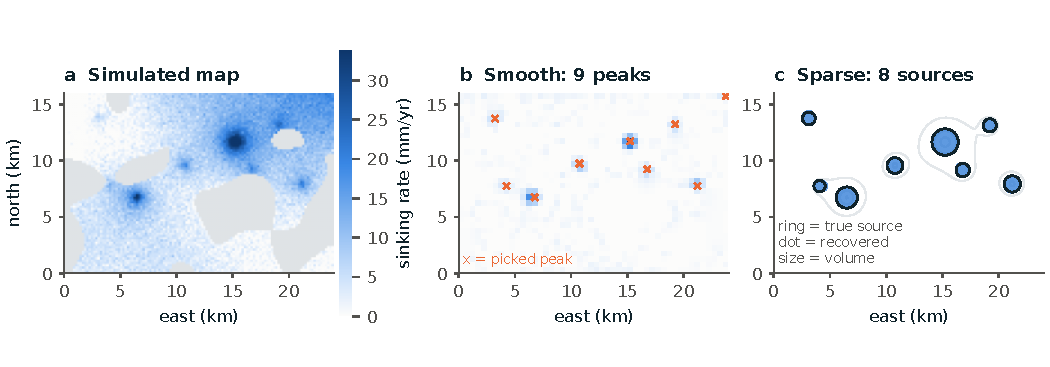
\includegraphics[width=\linewidth]{fig/example.pdf}
\caption{One of the \nScen\ maps. (a) What the radar would deliver; grey patches are missing data.
(b) The smooth baseline on its candidate grid. (c) The sparse result against the truth, with faint
contours of the true pumping signal. In this example both methods do well; across all maps the
smooth baseline produced \smNest\ peaks for \nTrue\ sources.}\label{fig:example}
\end{figure}

\subsection{Result 2: the uncertainty is honest}

\begin{itemize}
\item With $B$ known, \calCover\,\% of true volumes fall inside the stated 90\,\% range. That is
inside the 80--95\,\% band of check \V{7}.
\item The stability score separates real from false: its median is \calStabTp\ for true detections
and \calStabFp\ for false ones. Keeping only detections with stability of at least 0.8 raises
precision from \calPrecision\,\% to \calPrecisionStab\,\%, at the cost of recall falling from
\calRecall\,\% to \calRecallStab\,\%.
\item Small sources are not systematically missed: recall is \recallSmall\,\% for 40--80 \kcm,
\recallMid\,\% for 80--160 and \recallLarge\,\% for 160--400.
\end{itemize}

\begin{figure}[H]
\centering
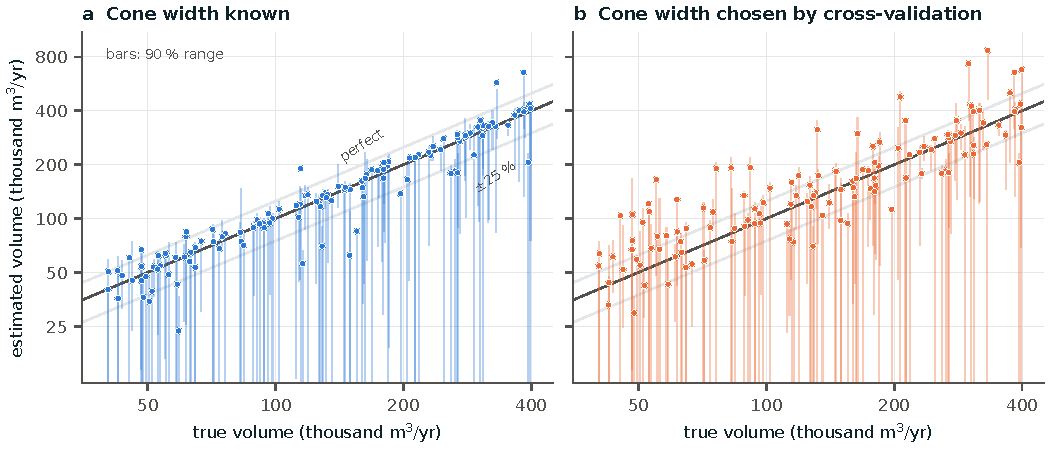
\includegraphics[width=\linewidth]{fig/volumes.pdf}
\caption{Estimated against true volume for every found source. (a) With the cone width known, points
hug the diagonal. (b) With the cone width chosen by cross-validation, whole maps shift up or down
together, because a wrong width rescales every source in that map.}\label{fig:volumes}
\end{figure}

\subsection{Result 3: where it breaks}

\begin{figure}[H]
\centering
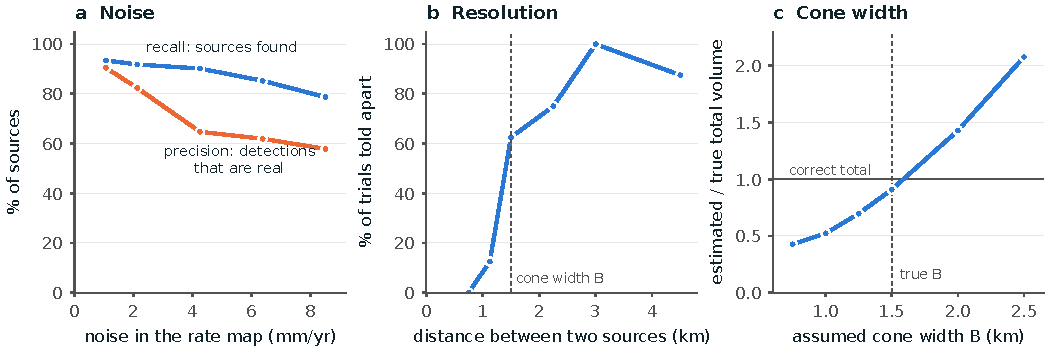
\includegraphics[width=\linewidth]{fig/limits.pdf}
\caption{Three limits, each from 8 maps per point with $B$ known in (a) and (b).
(a) More noise brings more false alarms. (b) Two equal sources of 200 \kcm\ are told apart only when
they are farther apart than about one cone width. (c) The estimated total volume grows with the
cone width that the analyst assumes.}\label{fig:limits}
\end{figure}

\textbf{Noise.} Table~\ref{tab:e2}. Recall stays high, but precision falls from \precNHalf\,\% at
\noiseHalf\,\mmyr\ to \precNTwo\,\% at \noiseTwo\,\mmyr. The stability filter becomes essential
there. Published Semarang maps report differences of 3--9\,\mmyr\ against GNSS \cite{azeriansyah2025,janur2025}, so careful quality control in \M{2} is
not optional.

\begin{table}[H]
\caption{Effect of noise ($B$ known).}\label{tab:e2}
\small\centering
\begin{tabular}{r r r r r}
\toprule
\textbf{Noise (\mmyr)} & \textbf{Recall (\%)} & \textbf{Precision (\%)} & \textbf{Volume error (\%)} & \textbf{Total}\\*
\midrule
\tabEtwo
\bottomrule
\end{tabular}
\end{table}

\textbf{Resolution.} Table~\ref{tab:e3}. Two sources closer than about one cone width (1.5\,km here)
are usually reported as one. The method resolves \emph{well fields}, not single wells. The merged
source still carries roughly the combined volume.

\begin{table}[H]
\caption{Telling two equal sources apart.}\label{tab:e3}
\small\centering
\begin{tabular}{r r r r}
\toprule
\textbf{Distance / $B$} & \textbf{Distance (km)} & \textbf{Told apart} & \textbf{Total}\\*
\midrule
\tabEthree
\bottomrule
\end{tabular}
\end{table}

\textbf{Cone width and shape.} Table~\ref{tab:e4}. This is the important one. If the analyst assumes
a cone half as wide as the true one, the total volume comes out at \totNarrow\ of the truth; with a
cone two-thirds wider, at \totWide. A Gaussian cone instead of the Bessel shape loses recall. In
contrast, detection is stable across widths from 1.0 to 2.5\,km (recall 85--86\,\%).

\begin{table}[H]
\caption{Effect of assuming the wrong cone (true: Bessel, $B = 1.5$\,km).}\label{tab:e4}
\small\centering
\begin{tabular}{l r r r r r}
\toprule
\textbf{Assumed shape} & \textbf{Width (km)} & \textbf{Recall (\%)} & \textbf{Precision (\%)} & \textbf{Volume error (\%)} & \textbf{Total}\\*
\midrule
\tabEfour
\bottomrule
\end{tabular}
\end{table}

\textbf{Can the data choose $B$ by itself?} Only roughly. Cross-validation picked the true 1.5\,km in
\cvBexact\ of \nScen\ maps and landed within 0.25\,km in \cvBnear. Its choices ranged from \cvBmin\ to
\cvBmax\,km. When it was right, the median volume error was \cvGoodErr\,\%; when it was wrong,
\cvBadErr\,\%. With $B$ from cross-validation, only \cvCover\,\% of true volumes fall inside the
stated range, below the pass band, because the bootstrap does not know that $B$ itself is uncertain.

\textbf{The ranking survives.} Even with a wrong cone width, the \emph{order} of sources is nearly
right. The rank correlation between true and estimated volumes is \rankCal\ with $B$ known, and
stays between \rankWide\ and \rankOneK\ for assumed widths from 0.75 to 2.5\,km.

\subsection{What we learned}

\begin{plain}
The inversion answers \emph{where} and \emph{in what order} reliably. It answers \emph{how much} only as
well as we know one number: the width of a pumping cone. So the audit should lead with the ranked
list, state volumes as a band across plausible cone widths, and narrow that band with well data.
\end{plain}

Four caveats about this experiment itself.
\begin{enumerate}
\item The same family of models made the data and inverted it. Table~\ref{tab:e4} relaxes this for
the cone, but not for everything else.
\item One cone width for the whole map. A real aquifer varies; a zoned $B$ is the natural extension.
\item Vertical motion was taken as given. Errors from stages \M{1}--\M{3} enter only as noise.
\item A snapshot in time. Sources that switch on or off (\M{4}) were not simulated.
\end{enumerate}

The code is in \texttt{code/}: \texttt{synth.py} (model and inversion), \texttt{run\_all.py} (the four
experiments), \texttt{analyze.py} (every number in this section) and \texttt{figures.py}.
